\documentclass[a4paper,nobalancelastpage]{revtex4-1}
\usepackage{amsmath,amssymb,graphicx,hyperref,mathtools, color, bm}
\usepackage{sidecap,subcaption}
\usepackage[labelfont=bf]{caption}
\usepackage[labelsep=space]{caption}
\usepackage[font={small}]{caption}
\usepackage{float}
\usepackage{listings}

\newcommand{\vect}[1]{\bm{#1}}
% Underlined vector format (bold, single underline)
\newcommand{\uvect}[1]{\bm{\underline{#1}}}
% Underlined matrix format (bold, double underline)
\newcommand{\umat}[1]{\bm{\underline{\underline{#1}}}}
\newcommand{\abs}[1]{\lvert #1 \rvert}
% Automatically expand cos into exponential -- note, pass both arguments positive
\newcommand{\cosexpansion}[2] {\frac{1}{2} \left[ e^{#1} e^{-#2} +e^{-#1}e^{#2} \right]}
\newcommand{\expn}[1] {e^{#1}}

\definecolor{singlemode}{RGB}{255, 153, 0}
\definecolor{multimode}{RGB}{0,178,148}

\newcommand{\smtitle}[1]{\textcolor{singlemode}{\textbf{#1}}}
\newcommand{\mmtitle}[1]{\textcolor{multimode}{\textbf{#1}}}

\graphicspath{{./figures/debug_log/}}

\usepackage[svgnames]{xcolor}
  \definecolor{diffstart}{named}{Grey}
  \definecolor{diffincl}{named}{Green}
  \definecolor{diffrem}{named}{OrangeRed}

\usepackage{listings}
  \lstdefinelanguage{diff}{
    basicstyle=\ttfamily\small,
    morecomment=[f][\color{diffstart}]{@@},
    morecomment=[f][\color{diffincl}]{+ },
    morecomment=[f][\color{diffrem}]{- },
  }

\begin{document}
\section*{Code \& debug log}

\mmtitle{1801121546} -- Running full code with interactions turned off because the alpha mod sq output yields a max val gaussian of $10^{-6}$ instead of order one for time interval 5 500 samples. Trying smaller time interval 0.05 500 samples yields even smaller peak $~3 \times 10^{-9}$.\\

\mmtitle{1801121619} -- Updated 1D code with last edits of full code, and running that to compare. Same problem as 1801121546.\\

\mmtitle{1801121720} -- Merged kernels branch and started new branch for current error. Isolated only the light equation, and only with the pump term.\\

\mmtitle{1801181419} -- Found fP=10 Delta0=1 yields a reasonable light field for just pump term, makes sense. \\

\mmtitle{1801181530} -- Steady state of $i\partial_t \alpha=\left[(\Delta_0-i \kappa) \alpha + f(r) \right]$ is $\alpha=f(r)/(\Delta_0-i \kappa)$, this matches if we do numerics with only this bit of eqn.\\

\mmtitle{1801221649} -- Reverted to the full equations of motion in 1D code and running that, with interactions turned off to check first and then with interactions on. \\

\mmtitle{1801311214} -- Wrote imaginary time code for 1D (in its own git branch), baffled by result.\\

\mmtitle{1802061355} -- Ran some code runs:
\begin{itemize}
\item long time 1D shows some persistent peaks, going longer and longer to check if it reaches a steady state, ran to 1000, 256 grid
\item full code for a long-ish time to match to 1D, 64 grid, seems alright but too choppy to tell
\end{itemize}

\smtitle{1802061418} -- (actually last week) ran singlemode time evo for a point below stability line but outside lin stab SR area, seems to be Normal state.\\

\mmtitle{1802061427} -- Running some more codes:
\begin{itemize}
\item longer 1D, 5000 time, lower res than 1802061355 (128 grid)
\item full code as 1802061355, but higher resolution to match 1D (128)
\end{itemize}

\mmtitle{1802091316} -- The 1D codes, clearly in 128 grid longer time, but also somewhat evident in 256 smaller interval, have as a steady state some pattern of peaks as in Fig. \ref{fig:1Dlong}.

\begin{figure}[H]
  \centering
  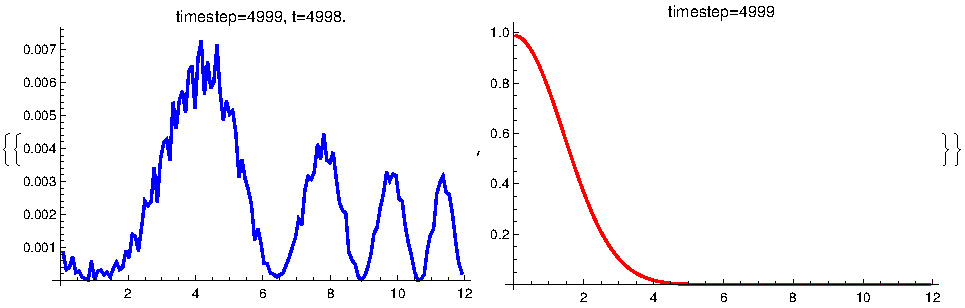
\includegraphics[width=5in]{1Dlongtimestate}
  \caption{Mod sq of atomic (blue) and light (red) fields for 1D  code run for a long time, folder: 1D\_ fP=1000\_ Delta0=100\_ N=1000\_ zA=0\_ epsilon=0\_ E0=50\_ 128-grid-LONGEST}
  \label{fig:1Dlong}
\end{figure}

The atomic field real and imaginary component for the same run are not well behaved, and both this behaviour and the 'steady state' behaviour is grid dependent:

\begin{figure}[H]
  \centering
  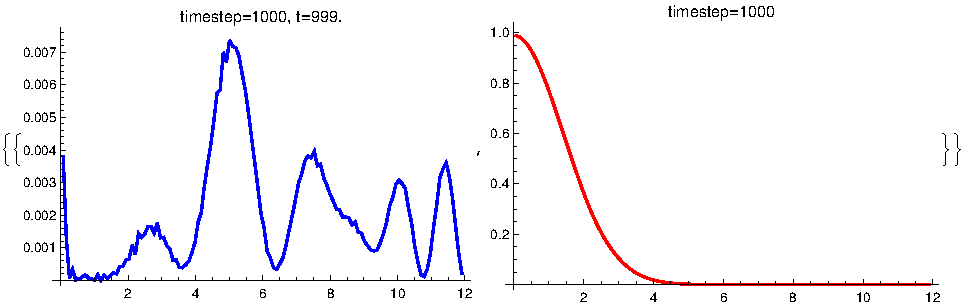
\includegraphics[width=5in]{1D-128-t1000-modsq}
  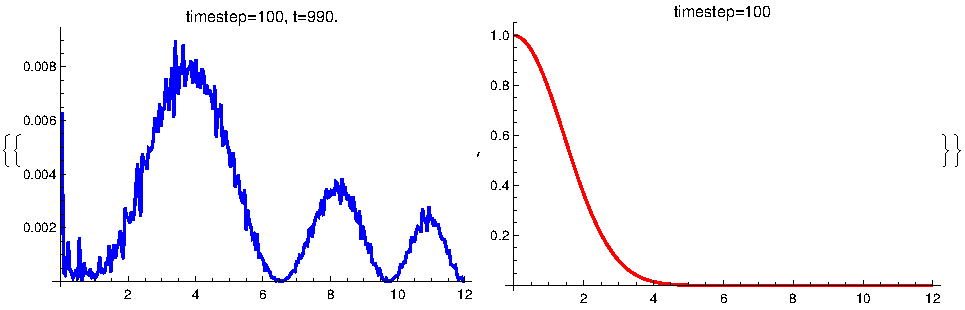
\includegraphics[width=5in]{1D-256-t1000-modsq}    
  \caption{Same time sample of mod sq atoms (blue) and mod sq light (red) for 128 (top) and 256 (bottom) grid}
  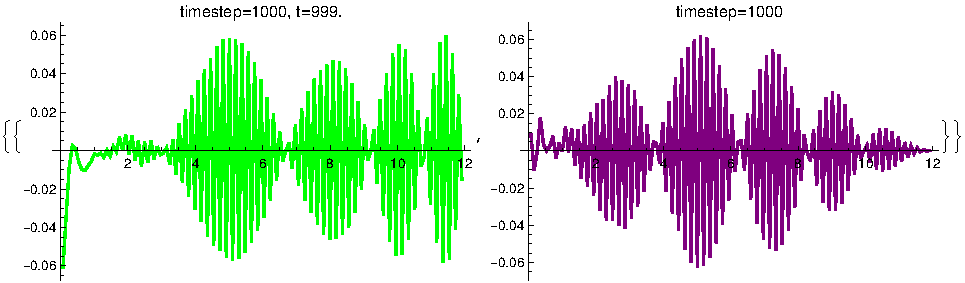
\includegraphics[width=5in]{1D-128-t1000-osc}
  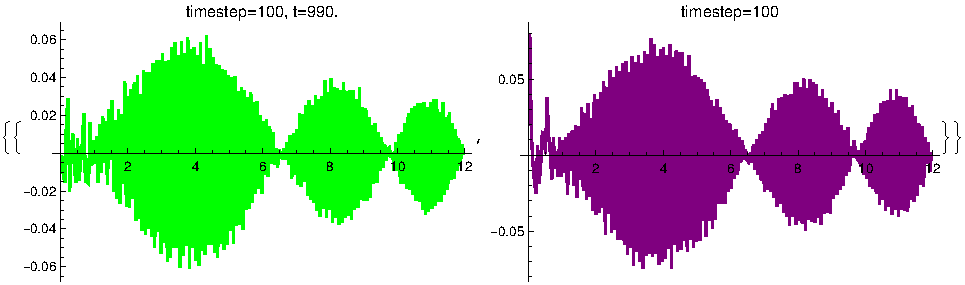
\includegraphics[width=5in]{1D-256-t1000-osc}    
  \caption{Same time sample of re atoms (green) and im atoms (purple) for 128 (top) and 256 (bottom) grid}
\end{figure}

light field and lightint (sample of convolution really) aren't too poorly behaved, e.g.

\begin{figure}[H]
  \centering
  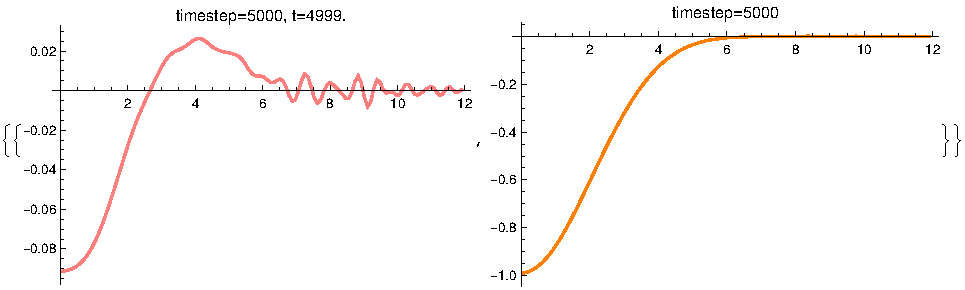
\includegraphics[width=5in]{1D-128-t5000-light}
    \caption{End time sample of re light (pink) and im light (orange) for 128 grid}
\end{figure}


\begin{figure}[H]
  \centering
   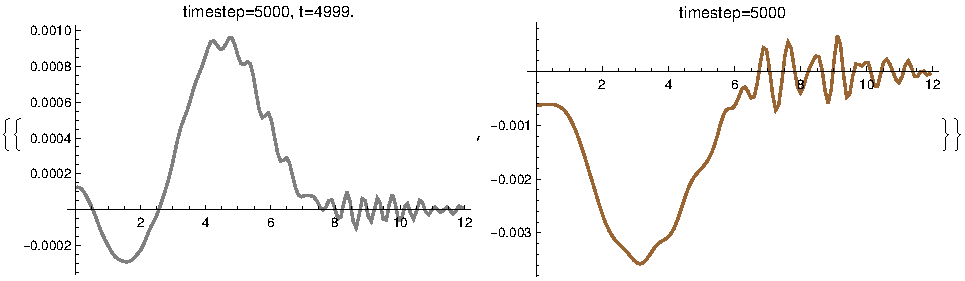
\includegraphics[width=5in]{1D-128-t5000-lightint}    
  \caption{Same time sample of re lightint (grey) and im lightint (brown) for 128 grid}
\end{figure}

Now need to a) look at full code if this matches vaguely b) figure out why atom eqn c) see if opposite detuning makes any sense

This is probably because after the initial quench, what happens to the dynamics is essentially they get projected on a number of high energy eigenstates which then evolve essentially independently, i.e. heating; these are high not only in real space but in momentum space, and therefore sensitive to grid cutoffs.\\

\mmtitle{1804091530} -- I was being daft, the multimode code first does the quench-bose nova thing, then above behaviour, i.e. we can carry on with adiabatically turning on pump (is this right?) i.e. balancing out the purely pump-dependent part of the effective potential on the atoms so we can circumvent the nova and watch for the effects of the interaction with light field.\\

\mmtitle{1805151420} -- Having updated the notes multimode-weak-coupling.tex, I want to code this in 1D -- pretty straightforward given that I already have a 1D integral kernel for the $U(r,r')$ term and the pump term for a large pump spot has a simple form that only depends on $r^2$ (see notes).

\noindent\rule{\textwidth}{0.5pt}\\
\\
\mmtitle{1808230000} -- Coded 1D weak coupling code.
\begin{itemize}
\item $f_P=1000$, $\Delta=-1000$, 10 time int, 100 steps too short for onset of oscillation.
\item Observing periodic oscillations for long time intervals (1000 time int, 100 steps) for negative detuning $f_P=1000$, $\Delta=-1000$.
\item Positive detuning $f_P=1000$, $\Delta=1000$ refuses to run past three steps -- WHY?
\end{itemize}

\mmtitle{1808231623} -- The oscillations which look periodic for $f_P=1000$, $\Delta=-1000$ do not actually have a constant period but look to be still settling (i.e. timestep 81 seems less periodic than timestep 101), however:
\begin{itemize}
\item $f_P=10000$, $\Delta=-1000$ refuses to run
\item $f_P=1000$, $\Delta=-1000$ time int=10000 very slow
\end{itemize}
Must understand why the ones which don't run don't run.\\
\\
\mmtitle{201808301119} -- Positive detuning sanity check, $f_P=10000$, $\Delta=1000$:
\begin{itemize}
\item for 1000 interval doesn't run
\item for 10 interval runs
\item for 100 interval: 
weak-coupling-realspace.cc:2063: WARNING: NaN present. Integration halted at t = 3.677196e+01.
Non-finite number in integration vector "atomicfield" in segment 1 $\rightarrow$ still Bose nova. Figure out why +ve detuning, and figure dependence on params for period.
\end{itemize}

\mmtitle{201809101130} -- (Not sure why I tried high pump first? Oh well)

Positive detuning figuring out: SHORT time interval first, $t_{max}=100$, $n_{steps}=100$.
\begin{itemize}
\item $fP=1, \ \Delta=1000$: runs IDENTICALLY to $fP=10$ and $fP=100$
\item $fP=1000, \ \Delta=1000$: breaks at TIME bose-nova like after oscillations which die out as peak grows
\end{itemize}

\mmtitle{201809111235} -- Am I being dumb? added potential and ran $fP=1000, \Delta_0=-1000, t_{max}=1000$, which are the params for which oscillations on non-pot code. With $\omega_{T}=1$ like old code, we get different behaviour (central spike, no notable oscillations). With *weaker* $\omega_{T}=0.01$ we get NaN at $tstep=5$, as well as with $\omega_T=0$ $\rightarrow$ figure out why setting Vext to zero isn't the same as taking it out ( which instead yielded the oscillatory results).

Using diff between the .xsil files of the results with oscillations (coming from the code without potential) and the results from the code with potential yields:

\begin{lstlisting}
184c184
<                   dpsi_dt= -i*( Ta[psi] - interaction*(Ureg+Uirr)*psi);
---
>                   dpsi_dt= -i*( Ta[psi]+Vext*psi - interaction*(Ureg+Uirr)*psi);
186c186
<          <dependencies>regularpart irregularpart</dependencies>
---
>          <dependencies>regularpart irregularpart externalpot</dependencies>
\end{lstlisting}

i.e. no substantial difference other than what we expect, but setting $\omega_{T}$ to zero in the potential code, both from run-realspace.sh and from within the code itself, yields the NaN error at tstep=5\\

\mmtitle{201809201549} -- Pulled JMJK changes (adding the longitudinal multimode code from other repo) and merged the correct (inc potential energy) branch so that main now contains the external energy term correctly, plus JMJK code.\\

\mmtitle{201809241013} -- Was being stupid setting $\omega_T-0$ instead of just potential term since $\omega_T$ is also in kinetic term. Now fixed, run $fP=1000, \Delta_0=-1000, t_{max}=1000$ -- reminder that this is the set of params that showed oscillations for the wrong (missing potential) code.\\

Sanity checks: if we set the potential energy term to zero then get the same oscillations for the same parameters. If we turn off interaction we have SHO oscillations, but also we can see that we already have numerical noise on data (the low amplitude fast wiggles) which tells us we should probably disregard these in future data.\\

With $E_0=0.01$ and $N=10000$, which I thought would be more reasonable params, $fP=1000, \Delta_0=-1000, t_{max}=1000$ yields very similar results to SHO - i.e. interaction not doing much.  Note that this is three orders of magnitude smaller than the $N=1000, E_0=1$ params we were running before.\\

\textbf{Running $N=10000, E_0=1$, $fP=1000, \Delta_0=-1000, t_{max}=1000$} -- if this does something interesting, then can check +ve detuning. \\

Also to be resolved in +ve: 
\begin{itemize}
\item Do the params for which interaction is weak (above) act consistently at +ve detuning ($E_0=0.01$ and $N=10000$ $fP=1000, \Delta_0=-1000, t_{max}=1000$);
\item NaN error on +ve det, e.g. at $fP=1000, \Delta_0=1000, t_{max}=100$ (NaN at tstep 1) or  $fP=100, \Delta_0=1000, t_{max}=100$ (NaN at tstep 80).
\end{itemize}
 To Be Cont'd, 1703\\

\mmtitle{201809261314} -- Cont'd from previous, positive detuning:
\begin{itemize}
\item Params for which interaction is weak do act consistently at +ve detuning ($E_0=0.01$ and $N=10000$ $fP=1000, \Delta_0=1000, t_{max}=1000$)

\item Setting $E_0=1$ for +ve detuning parameters above instead produces a NaN error right off the bat

\begin{verbatim}
weak-coupling-realspace.cc:2105: WARNING: NaN present. Integration halted at t = 7.249935e-01.
         Non-finite number in integration vector "atomicfield" in segment 1.
Sampled field (for moment group #1) at t = 7.249935e-01
Segment 1: minimum timestep: 3.076026e-289 maximum timestep: 1.000000e-01
  Attempted 16529 steps, 25.05% steps failed.
\end{verbatim}

\item Running $E_0=1$ with $N=10000$ $fP=1000, \Delta_0=1000, t_{max}=1000$ produces a NaN error after seven timesteps instead: SHO up to tstep=9 on tmax=100, then blows up -- run tmax=10 and see a) if onset changes b) if more info can be gotten before onset

\end{itemize}

Negative detuning:

\begin{itemize}
\item  $N=10000, E_0=1$, $fP=1000, \Delta_0=-1000, t_{max}=1000$ yields pretty noisy oscillations, wondering if it's artefact of sampling in spherical
\item running same as above but on 192 grid: same oscillations, don't seem to be sampling artefacts (check effect of 192 grid on SHO just to sanity check)
\end{itemize}

\mmtitle{201809261520} -- Now checking:
\begin{itemize}
\item effect of 192 vs 128 grid, tolerance: SHO noise is unchanged by lower tolerance or higher res, artefact of bessel transf
\item May be worth checking grid/tolerance effect on -ve detuning wiggles
\item positive detuning onset \& behaviour
\end{itemize}

\mmtitle{201809271131} -- positive detuning:
\begin{itemize}
\item Running tmax=10 for same params as tmax=100 causes it to hang instead of NaN; it also takes a long time to write output to file for some reason, and though I killed it at timestep 79 it only eventually wrong the first 70 timesteps to output
\item (Coding bafflement: I had to kill it from bg cos I had forgotten screen and more than 12h later it was still running, but the output got renamed like it finished -- probs killing it didn't kill script handler?)
\item Data produced isn't any more useful and matches tmax=100 up to breaking suddenly -- data is SHO up until suddenly spiking ($10^{205}$ in $tmax=100$ which NaNs) 
\end{itemize}


\mmtitle{201810011836} -- Found some mistakes and fixed them, as well as tidied up some equations in code for ease of reading. Below is the output of diff:

\lstinputlisting[language=diff]{20181001-changes-diff.txt}

Actual changes are just the missing 1/cos in the Ftheta term at  \texttt{@@ -104,9 +104,10 @@} , and interaction sign that means Delta0 influence should be switched at \texttt{@@ -182,7 +190,7 @@}. \\

\mmtitle{201810012012} -- Found another mistake:  at \texttt{@@ -134,10 +137,14 @@}, extra \* after Delta0's squared in prefactors -- and again in Uirr at \texttt{@@ -158,10 +165,11 @@}, fixed

\mmtitle{201810021111} -- Missing 1/cos term also had a spurious divided at  \texttt{@@ -104,9 +104,10 @@} , fixing this in old code (plus 1/cos term) should yield same result as corrected code.\\

\mmtitle{201810021203} -- Old code now produces qualitatively similar results (no NaN, oscillations for both detunings) but does not completely match new code, figure out why step by step by starting from old code, making changes until we match new.
\begin{enumerate}
\item Fixing $1/cos$ factor and spurious division in F in old cose fixes odd behaviour due to wrong division, behave similarly to new code but not matching;
\item Fixing remaining diff in F term: no change from (1)
\item Adding a and b real constants replacements in D2theta: no change from (1)
\item Made a,b double cos I got it wrong before, and matching bracketing to squash diff output for F: obviously no change (thankfully)
\item Changed prefactor definition in Urrp to match new code: no change from (1)
\item \textbf{Tidying up 2s in new code}: 1/2 in prefactor instead of 2/4 in both U's, and factor of 2 is right if we add the two FplusFminus and FminusFplus -- no change from new code results 
\item Changed $(FminusFplus+FplusFminus)$ to $2*Fplus*Fminus$ in old code: \textbf{this is what makes the difference} -- now positive detuning of old code matches negative detuning of new code and vice-versa (due to interaction change)
\end{enumerate}

\mmtitle{201820021320} -- Item (7) on debugging above is actually not due to $(FminusFplus+FplusFminus)$ changing wrt $2*Fplus*Fminus$, but to an extra factor of 2 in old code in Uirr: prefactor lacked a 1/2. Adding this mistake to new code yields the same result as items (1-5). New code is accepted. \\

\mmtitle{201810081110} -- Catch-up for work since 02/10. Having corrected the errors in previous log entries, we get output that shows instability that is quaitatively similar for both detunings. To understand this: strip all 'extra' parts (gaussian initialisation, harmonic trap) and have just a flat distribution with the interaction.\\

Running this in radial coordinate 1D simulation picks out a peak at the centre, which makes no sense because it shouldnt be preferred to any other point due to boundary conditions \& flat distribution $\rightarrow$ try coding this in plain 1D (no bessel)\\

Several batches of results:
\begin{enumerate}
\item 1D non-bessel flat distribution
\begin{enumerate}
\item $fP=100, \Delta_0=\pm 1000$
\item $fP=1000, \Delta_0=\pm 1000$
\item $fP=10000, \Delta_0=\pm 1000$
\end{enumerate}
\item 1D non-bessel gaussian distribution, no trap
\begin{enumerate}
\item $fP=100, \Delta_0=\pm 1000$
\item no interaction (parameters irrelevant)
\item $fP=1000, \Delta_0=\pm 1000$
\item $fP=10000, \Delta_0=\pm 1000$
\end{enumerate}
\item ``full" 1D non-bessel, gaussian dist and harmonic trap
\begin{enumerate}
\item $fP=1000, \Delta_0=\pm 1000$
\item $fP=10000, \Delta_0=\pm 1000$
\end{enumerate}
\item original, radial code, flat distr, no trap
\item original, radial code, Gaussian distr, no trap
\item "full" original, radial code, Gaussian distr, harmonic trap
\end{enumerate}

\textbf{Observations:}\\

(1.a) detunings are different but not qualitatively depending on range/grid $\rightarrow$ understand better\\

(1.b) \\

(2.a) is the same as (2.b); results are range dependent but not grid dependent $\rightarrow$ try higher pump strength\\

(2.c) shows roughly opposite behaviour for opposite detuning (+ve repulsive, -ve attractive) but some difference in range/grid spacing (particularly baffling difference between +ve range 24 grid 128/256)\\

(2.d) similar to (2.c) but more marked\\

(3.a) both detunings the same\\

(3.b) detunings different, -ve attractive, +ve repulsive, but grid and range dependent, understand better\\

\mmtitle{201810151718} -- Things to check:

\begin{enumerate}
\item Gaussian distribution full (3.b) from above: 24 range 256 grid is the same as 12 range 128 grid, i.e. grid spacing dependent
\item Flat distribution at higher pump powers:
\item Analytic form of long-range interaction:
\item Control short range and long range components of interactions separately, see if this makes sense with what we're seeing, i.e. Gaussian sees mostly/only short range,
\end{enumerate}


%%%%%%%%%%%%%%%%%%%%%%%%%%%
% COMMENTED OUT STUFF

\iffalse
FUTURE TABLES =============
+ve detuning:

\begin{center}
\begin{tabular}{ | c | c | c | c | } 
 \hline
 $f_P$ & c$\Delta_0$ & $t_{max}$ & results \\ 
\hline
 10 & 1000 & 100 & \\ 
 100 & 100 & 100 & \\ 
  100 & 1000 & 100 & \\ 
 \hline
\end{tabular}
\end{center}

-ve detuning:

\begin{center}
\begin{tabular}{ | c | c | c | c | } 
 \hline
 $f_P$ & c$\Delta_0$ & $t_{max}$ & results \\ 
\hline
 100 & -100 & 100 & \\ 
 100 & -1000 & 100 & \\ 
  1000 & -1000 & 100 & \\ 
 \hline
\end{tabular}
\end{center}
\fi


\end{document}